\section{Web-based Demo System}
In order to better illustrate the work that has been done in this final year project, a web-based demo system is also implemented based on Django, which is a popular python web framework. There are generally two components for web application: back end and front end, where front end is responsible to collect data from users and process it to conform the requirements of back end, and back end processes the received data. Back to this demo system, Django adopts previous python modules like extracting SIFT features and calculating EMD distance as the back end side. For the front end, a CSS library called Bootstrap is used for better visualization. Also, ajax is heavily used to connect the user input with the back end server and dynamically update the web page. \\

\begin{figure}[!ht]
\centering
	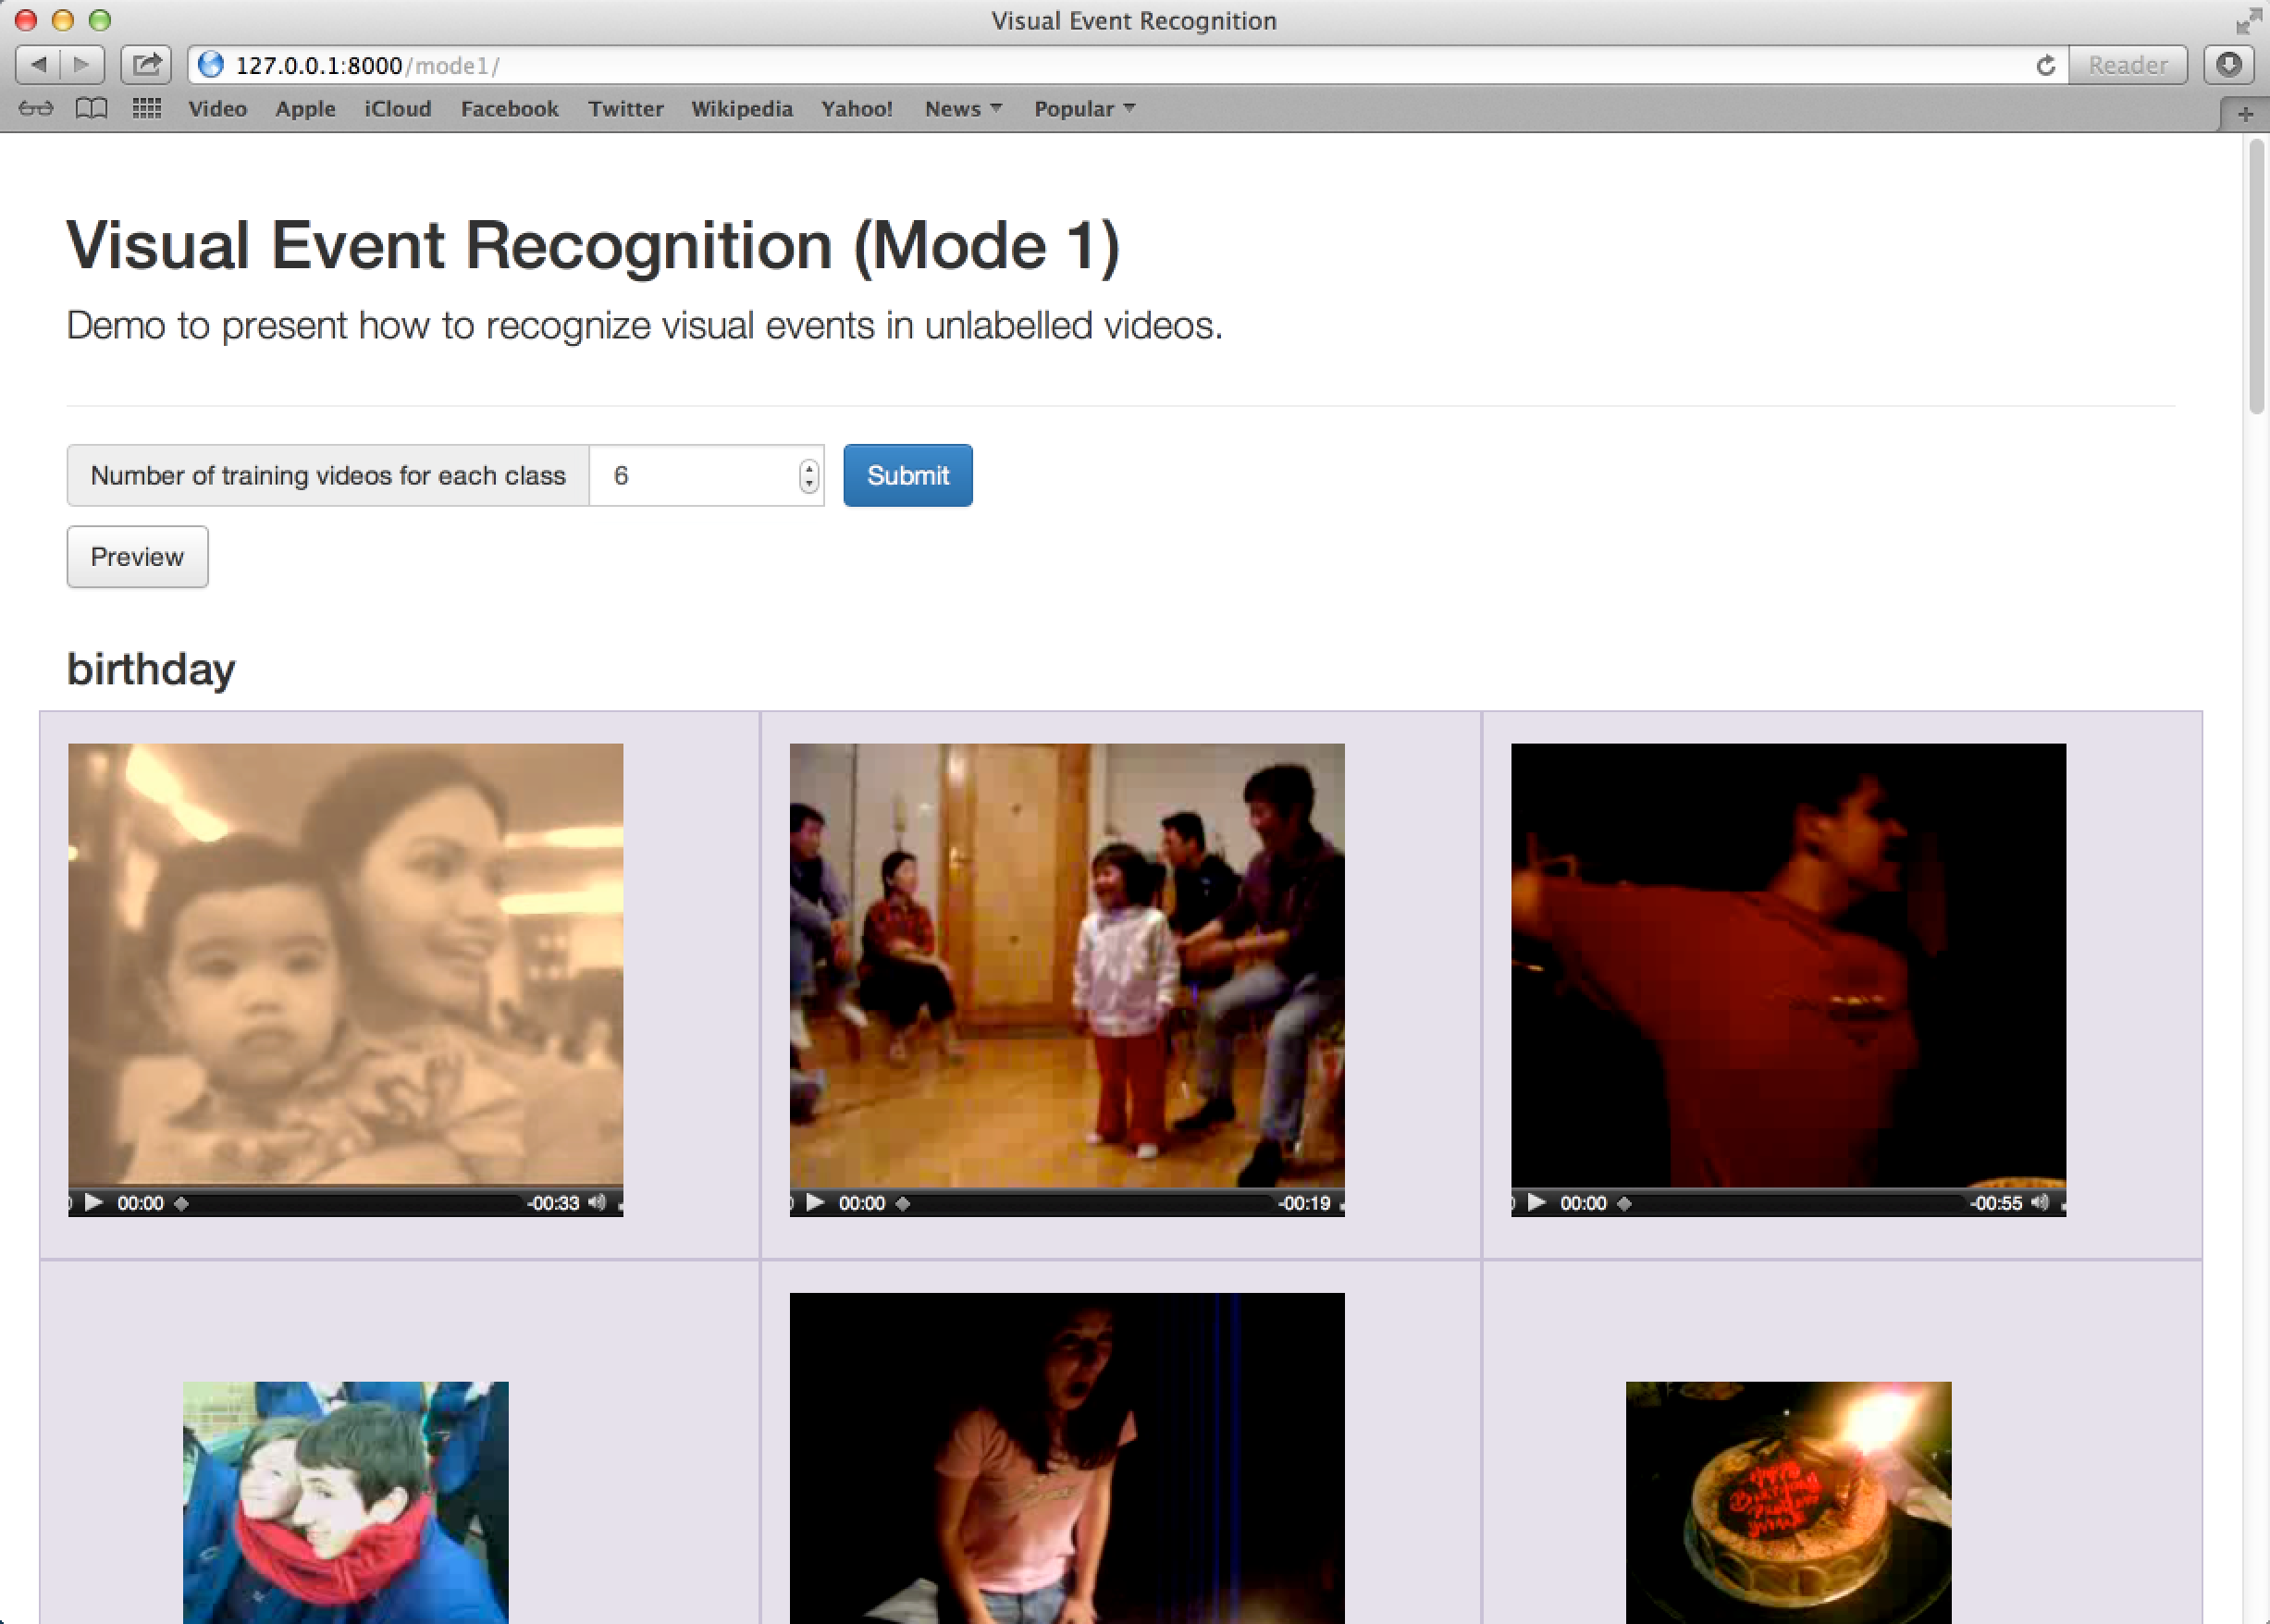
\includegraphics[scale=0.2]{./mode1.png}
\caption{Snapshot of mode 1. In mode 1, the distance matrix of Youtube videos is calculated offline. The user could randomly select the training data and testing data to check the recognition performance.}
\end{figure}

\begin{figure}[!ht]
\centering
	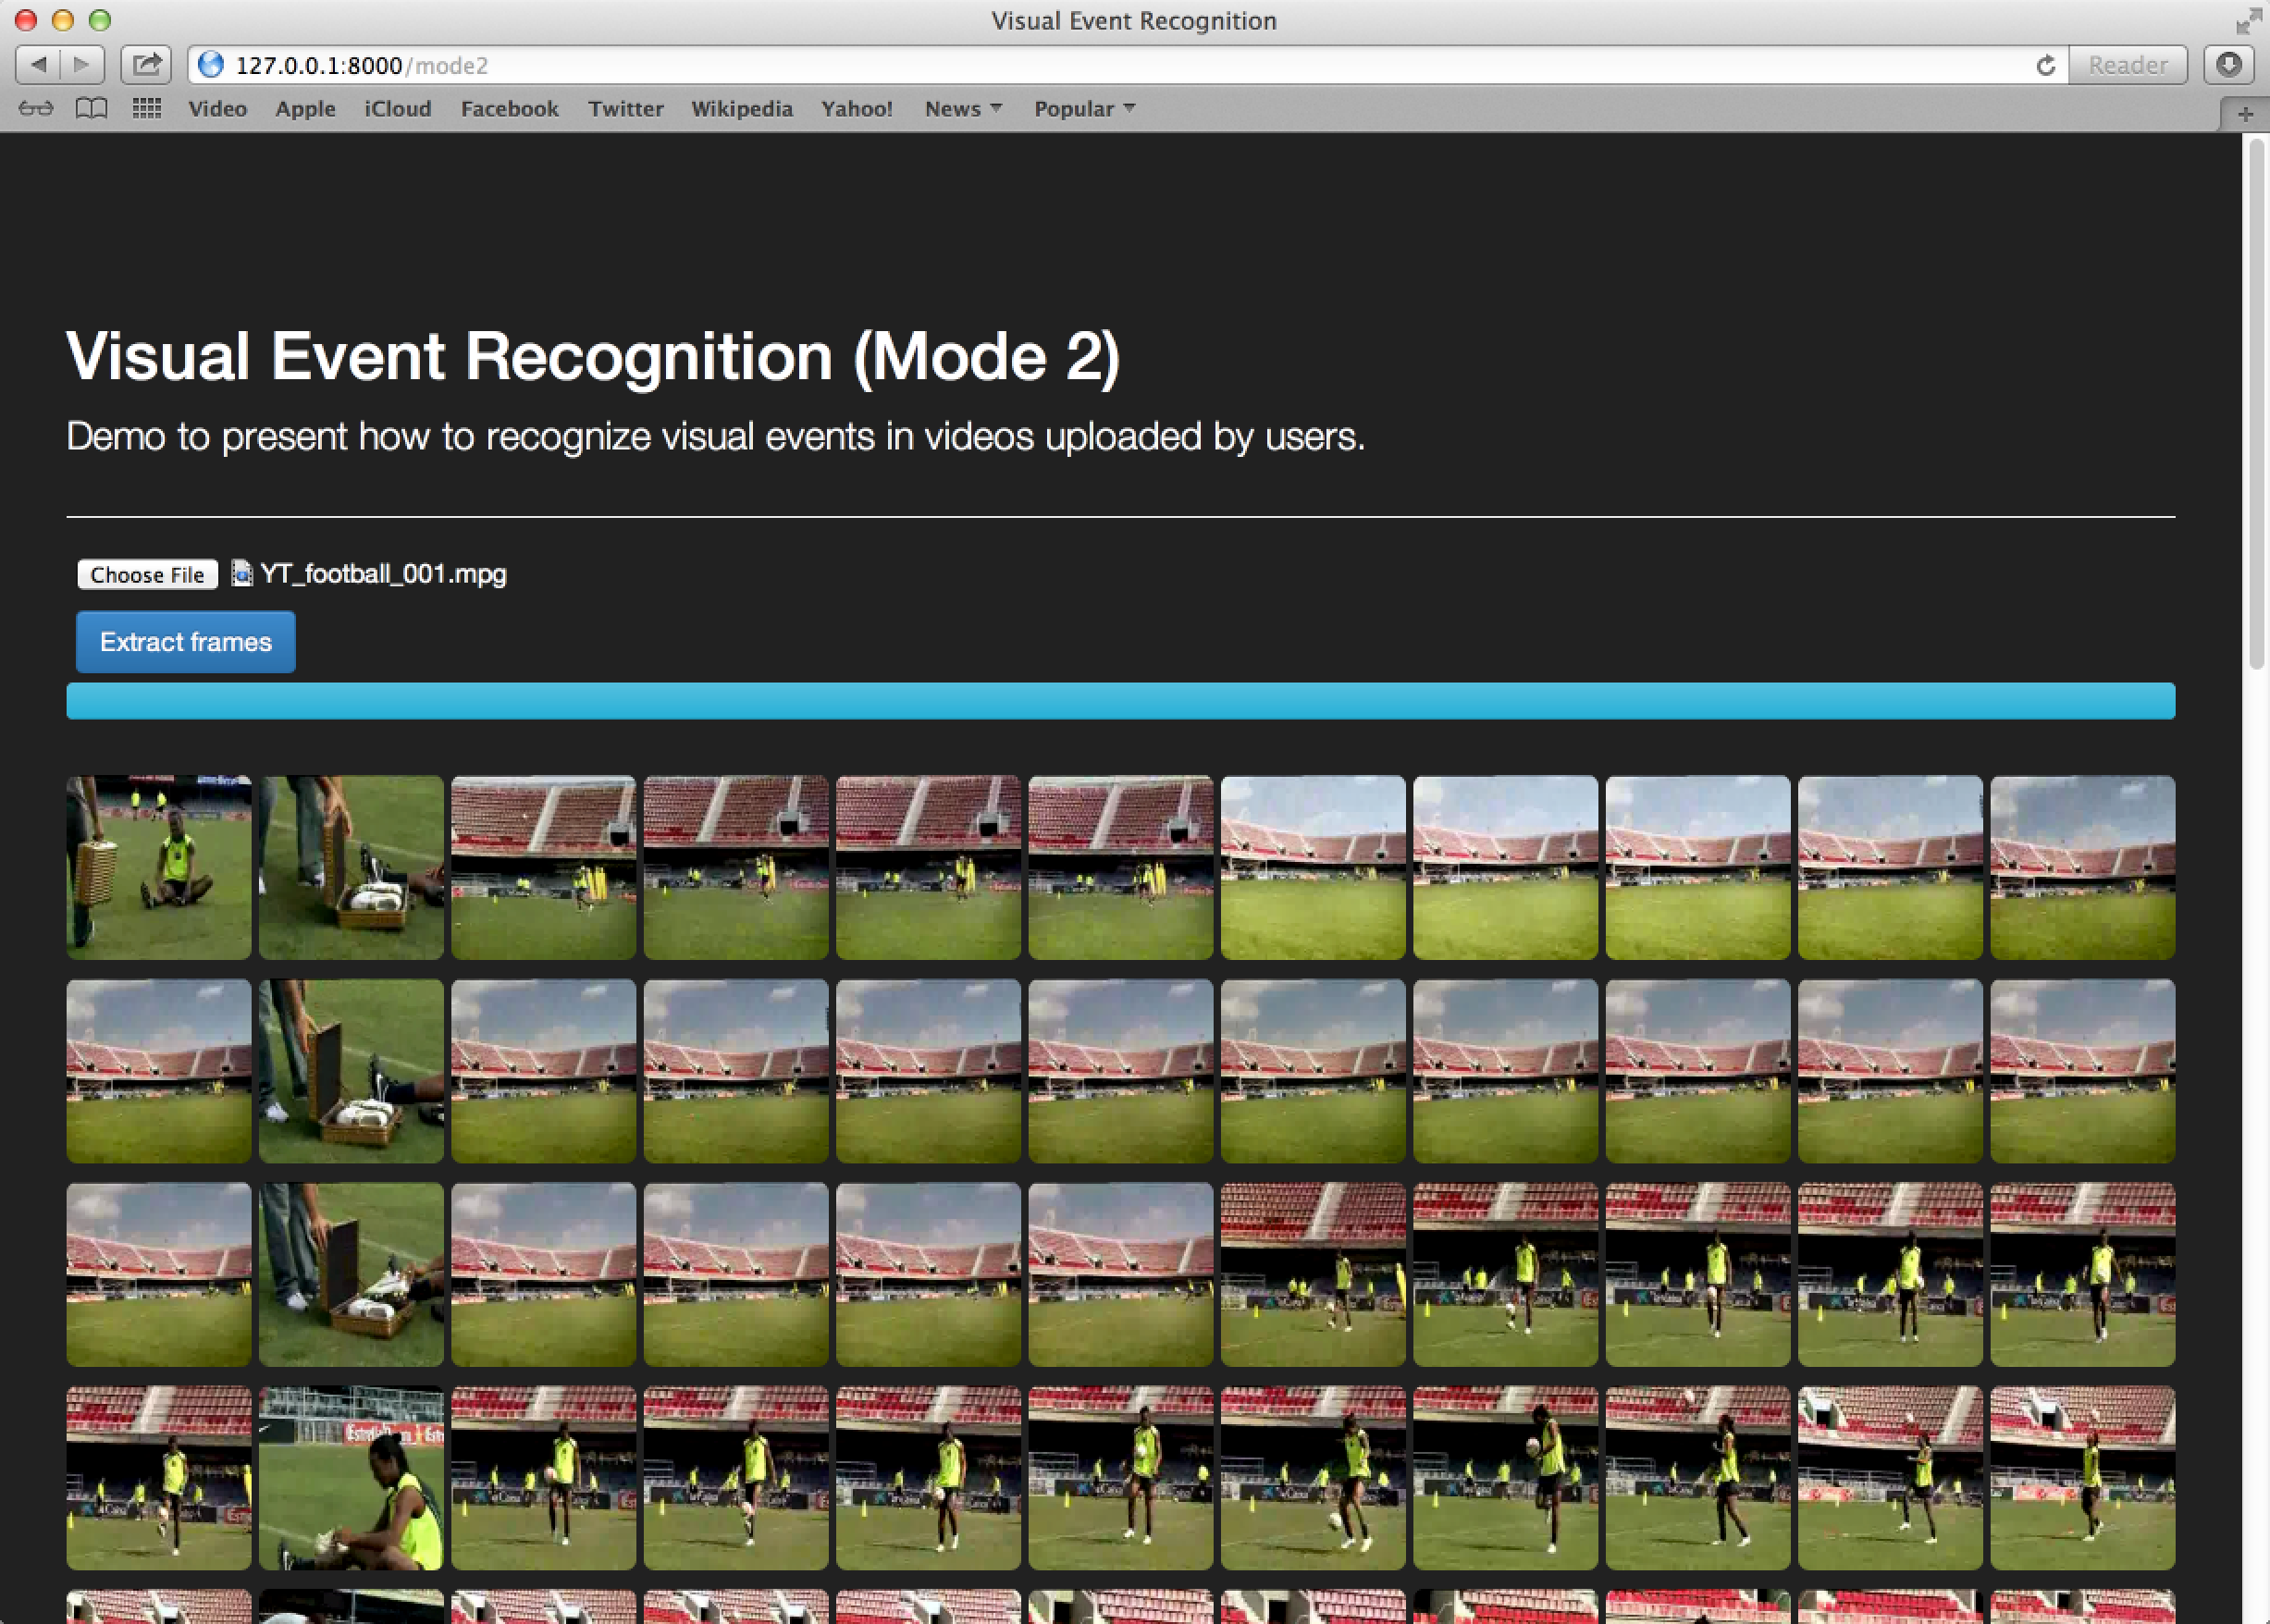
\includegraphics[scale = 0.2]{./mode2.png}
\caption{Snapshot of mode 2. In mode 2, the user could upload a new video and get the label of this video predicted by the underlying recognition system}
\end{figure}

\noindent There are two modes built for two different purposes as shown in Figure 18 and 19, respectively. 
\begin{itemize}
	\item{\bf Mode 1} \\
	Mode 1 enables the user to randomly select training and testing Youtube videos for recognition. The distance matrix used in recognition is calculated offline to save time. The procedures go as following. Firstly, the user selects the number of videos per class as training data. Secondly, the classifier based on the training data is built. Thirdly, recognitions on the rest of videos are performed using the classifier built in the previous step. Lastly, in the result section, not only the recognition accuracy is displayed, but also a confusion matrix, which better visualizes the performance.   

	\item{\bf Mode 2} \\
	The second mode aims to present users the whole process of recognizing videos. The user could upload a new video and check how this video is recognized from extracting frames, extracting features and building histograms all the way down to calculating distances with training videos and building a classifier for recognition. Such interactive presentation shall give users a clear idea about video recognition.
\end{itemize}

\noindent To conclude, this web-based demo system presents visual event recognition in two modes nicely. Following the procedures, users shall be able to understand the underlying operations to recognize videos. 






